\documentclass{article}
\usepackage{graphicx}% Required for inserting images
\usepackage{lindrew}
\usepackage{pdfpages}
\usepackage[shortlabels]{enumitem}
\usepackage{matlab-prettifier}
\usepackage{algorithm}
\usepackage{algpseudocode}

\title{ACM 104 Problem Set 3}
\author{Amitesh Pandey}
\date{October 2024}
\begin{document}
\maketitle
\section*{Problem 1: Inner Products vs Norms}
(a) We need to show that we can construct the arbitrary inner produce $\langle u, v\rangle$ using only the norms of some vectors. 
\begin{equation*}
    ||u + v|| = \sqrt{\langle u + v, u + v \rangle}
\end{equation*}
Then we have
\begin{equation*}
    ||u + v||^2 = \langle u + v, u + v \rangle
\end{equation*}
On expanding the right hand
\begin{equation*}
    ||u + v||^2 = \langle u + v, v \rangle + \langle v, u + v \rangle = \langle u, v\rangle + \langle v, v\rangle + \langle v, u\rangle + \langle v, v \rangle = \langle u, u\rangle + 2\langle u, v \rangle + \langle v, v \rangle
\end{equation*}
Now we know $\langle u, u\rangle = ||u||^2, \langle v, v \rangle = ||v||^2$, so we get for $\langle u, v \rangle$, 
\begin{equation*}
    \langle u, v \rangle = \frac{||u + v||^2 - ||u||^2 - ||v||^2}{2}
\end{equation*}
(b) We will show that two inner products that induce the same norm must necessarily be non-distinct. Assume for any $u,v$, that the norms are
\begin{equation*}
    ||u||_{1} = ||u||_{2}, ||v||_{1} = ||v||_{2} \implies \langle u, u\rangle_{1} = \langle u, u\rangle_{2},\langle v, v\rangle_{1} = \langle v, v\rangle_{2}
\end{equation*}
for some inner products $\langle u, u \rangle_{1},\langle u, u\rangle_{2}$. Now consider the sum such that
\begin{equation*}
    \langle u + v, u + v \rangle_{1} = \langle u, u\rangle_{1} + 2\langle u, v \rangle_{1} + \langle v, v \rangle_{1}
\end{equation*}
\begin{equation*}
    \langle u + v, u + v \rangle_{2} =  \langle u, u\rangle_{2} + 2\langle u, v \rangle_{2} + \langle v, v \rangle_{2}
\end{equation*}
By assumption $||u+v||_{1} = ||u+v||_{2}$, we must also have
\begin{equation*}
    \langle u, u\rangle_{1} - \langle u, u\rangle_{2} + 2\langle u,v\rangle_{1} - 2\langle u, v\rangle_{2} + \langle v, v\rangle_{1} - \langle v, v\rangle_{2} = 0
\end{equation*}
Then we simply get $\langle u, v\rangle_{1} = \langle u, v\rangle_{2}$. Thus these are the same inner products for all arbitrary $u,v$.
\newpage
\section*{Problem 2: Continuously Differentiable Functions}
(a) Notice for the first inner product $\langle f, g\rangle_{1}$ that if the inner product $\langle f, f\rangle_{1} = k$ for any $k \neq \mathbf{0} \in \mathbb{R}^{n}$ then it follows that
\begin{equation*}
    \langle f, f\rangle_{1} = \int_{0}^{1} f'(x)f'(x)\text{d}x = \int_{0}^{1} 0\cdot 0\text{d}x = 0
\end{equation*}
But we know that $\langle f, f\rangle_{1} \neq 0$ unless $f = \mathbf{0}$, thus this isn't positive definite. Since the first one isn't an inner product, and one of them has to be an inner product as per the question, we conclude that it's the second one. \\\\
(b) Let $f$ and $g$ be two functions, then the inner product
\begin{equation*}
    \langle f, g\rangle = \int_{0}^{1}(fg + f'g')\text{d}x
\end{equation*}
obeys the following Cauchy-Schwartz Inequality:
\begin{equation*}
    |\langle f, g \rangle |^2 \leq \langle f,f \rangle \cdot \langle g, g\rangle 
\end{equation*}
Now by definition, we have
\begin{align*}
    \langle f, f\rangle &= \int_{0}^{1}(f^2 + f'^2)\text{d}x\\
    \langle g, g\rangle &= \int_{0}^{1}(g^2 + g'^2)\text{d}x
\end{align*}
Thus we have
\begin{equation*}
    |\langle f, g\rangle |^2 \leq \left(\int_{0}^{1}(f^2 + f'^2)\text{d}x\right)\cdot \left(\int_{0}^{1}(g^2 + g'^2)\text{d}x\right)
\end{equation*}
It also obeys the following Triangle inequality:
\begin{equation*}
    ||\langle f + g, f + g \rangle|| \leq ||\langle f, f\rangle || + ||\langle g,g\rangle ||
\end{equation*}
Note that 
\begin{equation*}
    ||\langle f + g, f + g\rangle || = \sqrt{\langle f + g, f + g \rangle} = \sqrt{\int_{0}^{1}((f+g)^2 + (f' + g')^2)\text{d}x}
\end{equation*}
So finally we have
\begin{equation*}
    \sqrt{\int_{0}^{1}((f+g)^2 + (f' + g')^2)\text{d}x} \leq \sqrt{\left(\int_{0}^{1}(f^2 + f'^2)\text{d}x\right)} + \sqrt{\left(\int_{0}^{1}(g^2 + g'^2)\text{d}x\right)}
\end{equation*}
(c) For this part, recall that for two elements $f,g \in C^{1}[0,1]$, the angle between them with respect to an inner product $\langle  -,- \rangle$ is given by
\begin{equation*}
    \theta = \cos^{-1}{\left(\frac{\langle f, g\rangle}{||\langle f,f \rangle||\cdot||\langle g,,g \rangle||}\right)} = \cos^{-1}{\left(\frac{\int_{0}^{1}e^{x}\text{d}x}{\left(\sqrt{\int_{0}^{1}1\text{d}x}\right)\cdot \left(\sqrt{\int_{0}^{1}2e^{2x}\text{d}x}\right)}\right)} = \cos^{-1}\left(\frac{e-1}{\sqrt{e^2 - 1}}\right) = \cos^{-1}(0.68) \approx 47^{\circ}
\end{equation*}
\newpage
\section*{Problem 4:  Gram Matrices}
(a) The Gram matrix $G$ of $v_{1}, v_{2}, \dots v_{n}$ in an inner product space with the inner product $\langle-,-\rangle$ is given by
\begin{equation*}
    g_{ij} = \langle v_{i}, v_{j}\rangle
\end{equation*}
Thus for $1, e^x, e^{2x}$, we obtain
\begin{equation*}
    G = \begin{pmatrix}
        \langle 1, 1\rangle & \langle 1, e^x \rangle& \langle 1, e^{2x}\rangle\\
        \langle e^{x},1 \rangle& \langle e^{x} ,e^{x} \rangle&\langle e^{x}, e^{2x}\rangle \\
        \langle e^{2x}, 1\rangle& \langle e^{2x}, e^x \rangle&\langle e^{2x}, e^{2x}\rangle
    \end{pmatrix}
\end{equation*}
When the inner product is $L^2$, we get
\begin{equation*}
    G = \begin{pmatrix}
        \int_{0}^{1} 1\text{d}x & \int_{0}^{1} e^{x}\text{d}x& \int_{0}^{1} e^{2x}\text{d}x\\
        \int_{0}^{1} e^{x}\text{d}x& \int_{0}^{1} e^{2x}\text{d}x&\int_{0}^{1} e^{3x}\text{d}x\\
        \int_{0}^{1} e^{2x}\text{d}x& \int_{0}^{1} e^{3x}\text{d}x&\int_{0}^{1} e^{4x}\text{d}x
    \end{pmatrix} = \begin{pmatrix}
        1 & e - 1 & \frac{e^2 - 1}{2}\\
        e - 1 & \frac{e^2 - 1}{2} & \frac{e^3 - 1}{3}\\
         \frac{e^2 - 1}{2} & \frac{e^3 - 1}{3} & \frac{e^4 - 1}{4}
    \end{pmatrix}
\end{equation*}
(b) The Gram matrix is positive-definite when the elements involved in it are linearly independent, since $1, e^{x}, e^{2x}$ are obviously linearly independent, $G$ in this case, is positive-definite.\\\\
(c) Using the inner product in problem (2), we have
\begin{equation*}
    G = \begin{pmatrix}
        \int_{0}^{1} 1\text{d}x & \int_{0}^{1} e^{x}\text{d}x& \int_{0}^{1} e^{2x}\text{d}x\\
        \int_{0}^{1} e^{x}\text{d}x& \int_{0}^{1} 2e^{2x}\text{d}x&\int_{0}^{1} 3e^{3x}\text{d}x\\
        \int_{0}^{1} e^{2x}\text{d}x& \int_{0}^{1} 3e^{3x}\text{d}x&\int_{0}^{1} 5e^{4x}\text{d}x
    \end{pmatrix} = \begin{pmatrix}
        1 & e - 1 & \frac{e^2 - 1}{2}\\
        e - 1 & e^2 - 1 & e^3 - 1\\
         \frac{e^2 - 1}{2} & e^3 - 1 & 5\frac{e^4 - 1}{4}
    \end{pmatrix}
\end{equation*}
Since $(1, e^x, e^{2x})$ are still linearly independent, $G$ is positive definite. \\\\
(d) The linear independence of $1, e^x, e^{2x}$ is invariant of the inner product the space is under, so as long as these are the elements involved in $G_1$ and $G_2$, they will both have to be positive-definite. 
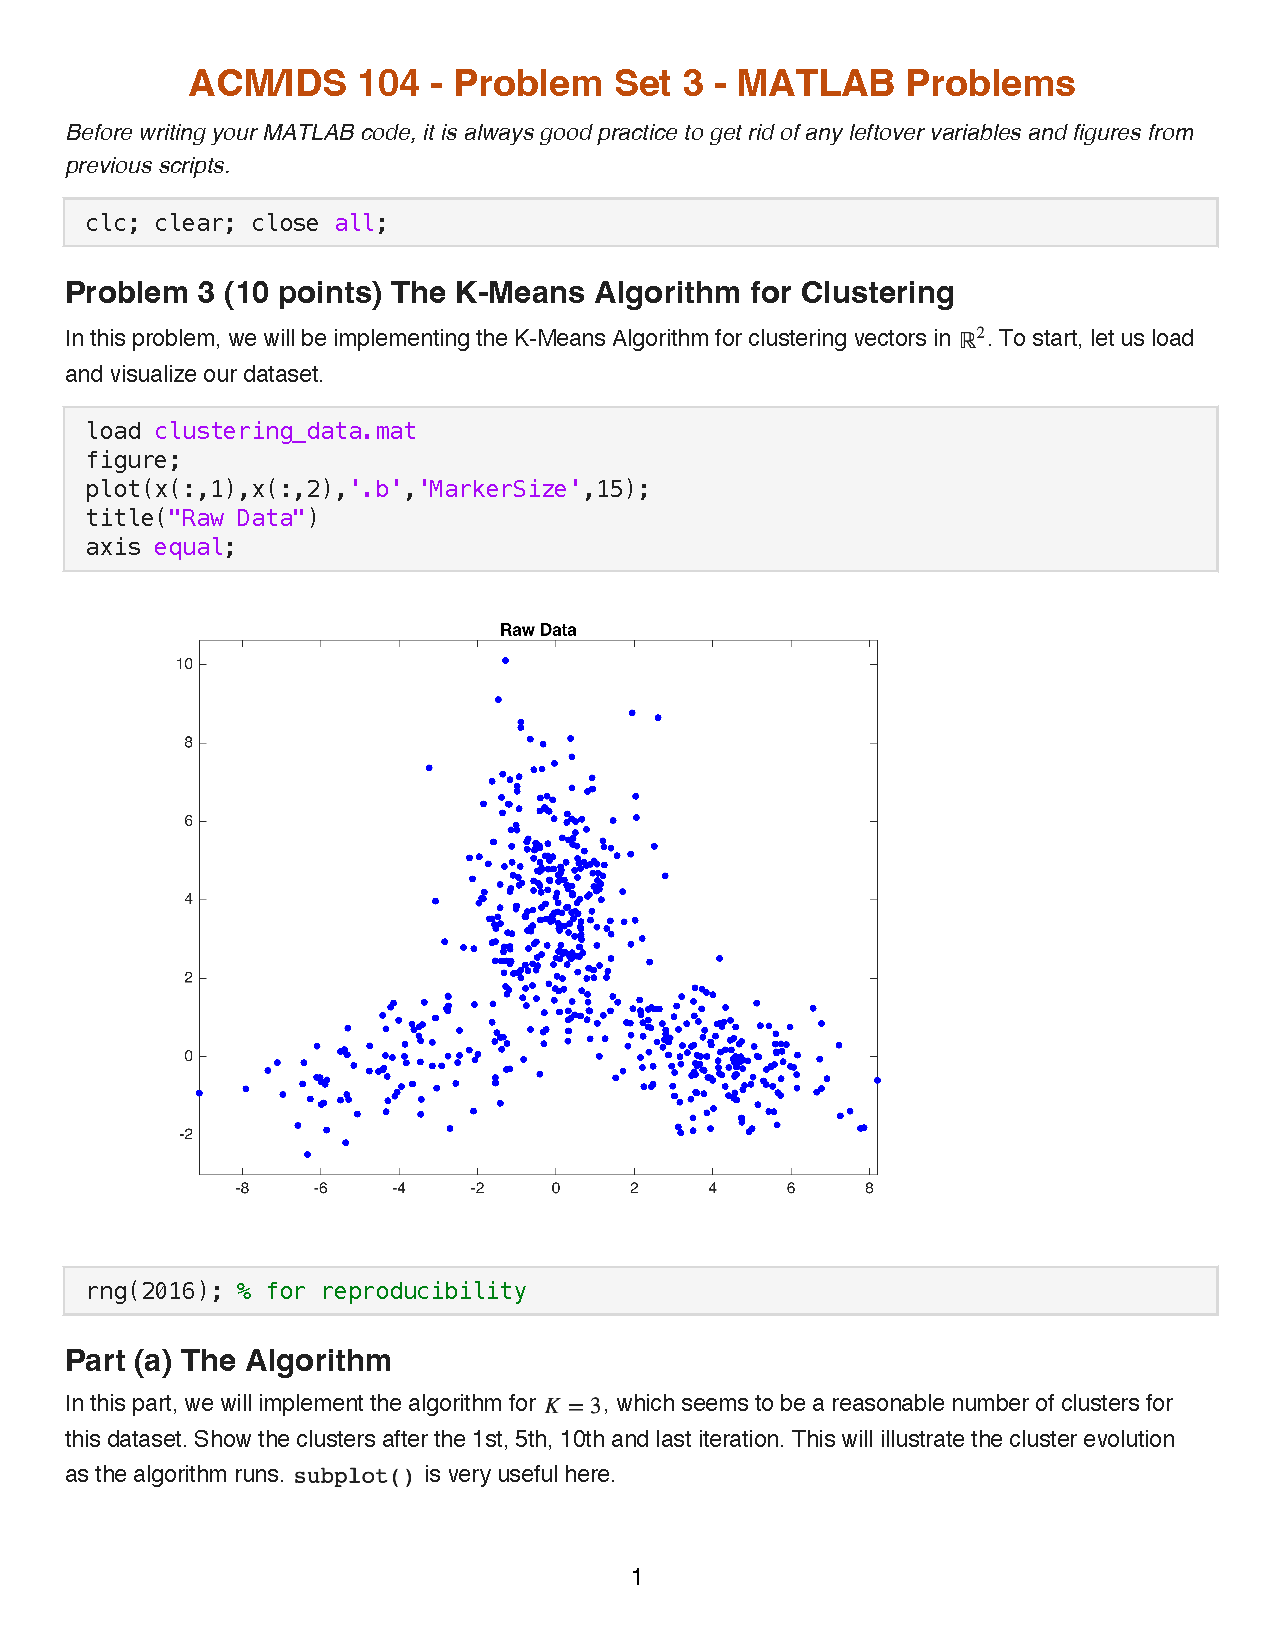
\includepdf[pages=-]{PS3matlab.pdf}



\end{document}
